\section{Resultados}

\begin{frame}{Recapitulacion de Objetivos}
    \vspace{0.2cm}
    \begin{itemize}
        \item Obtener una implementacion integrada en \texttt{PyTorch}
        \item Mantener fiabilidad numerica con el modelo de Ariel
        \item Aplicar algun metodo de entrenamiento estandar de DeepRl
        \item Resolver un problema de control continuo
    \end{itemize}
\end{frame}

\begin{frame}{Equivalencia Numerica}
    \centering
    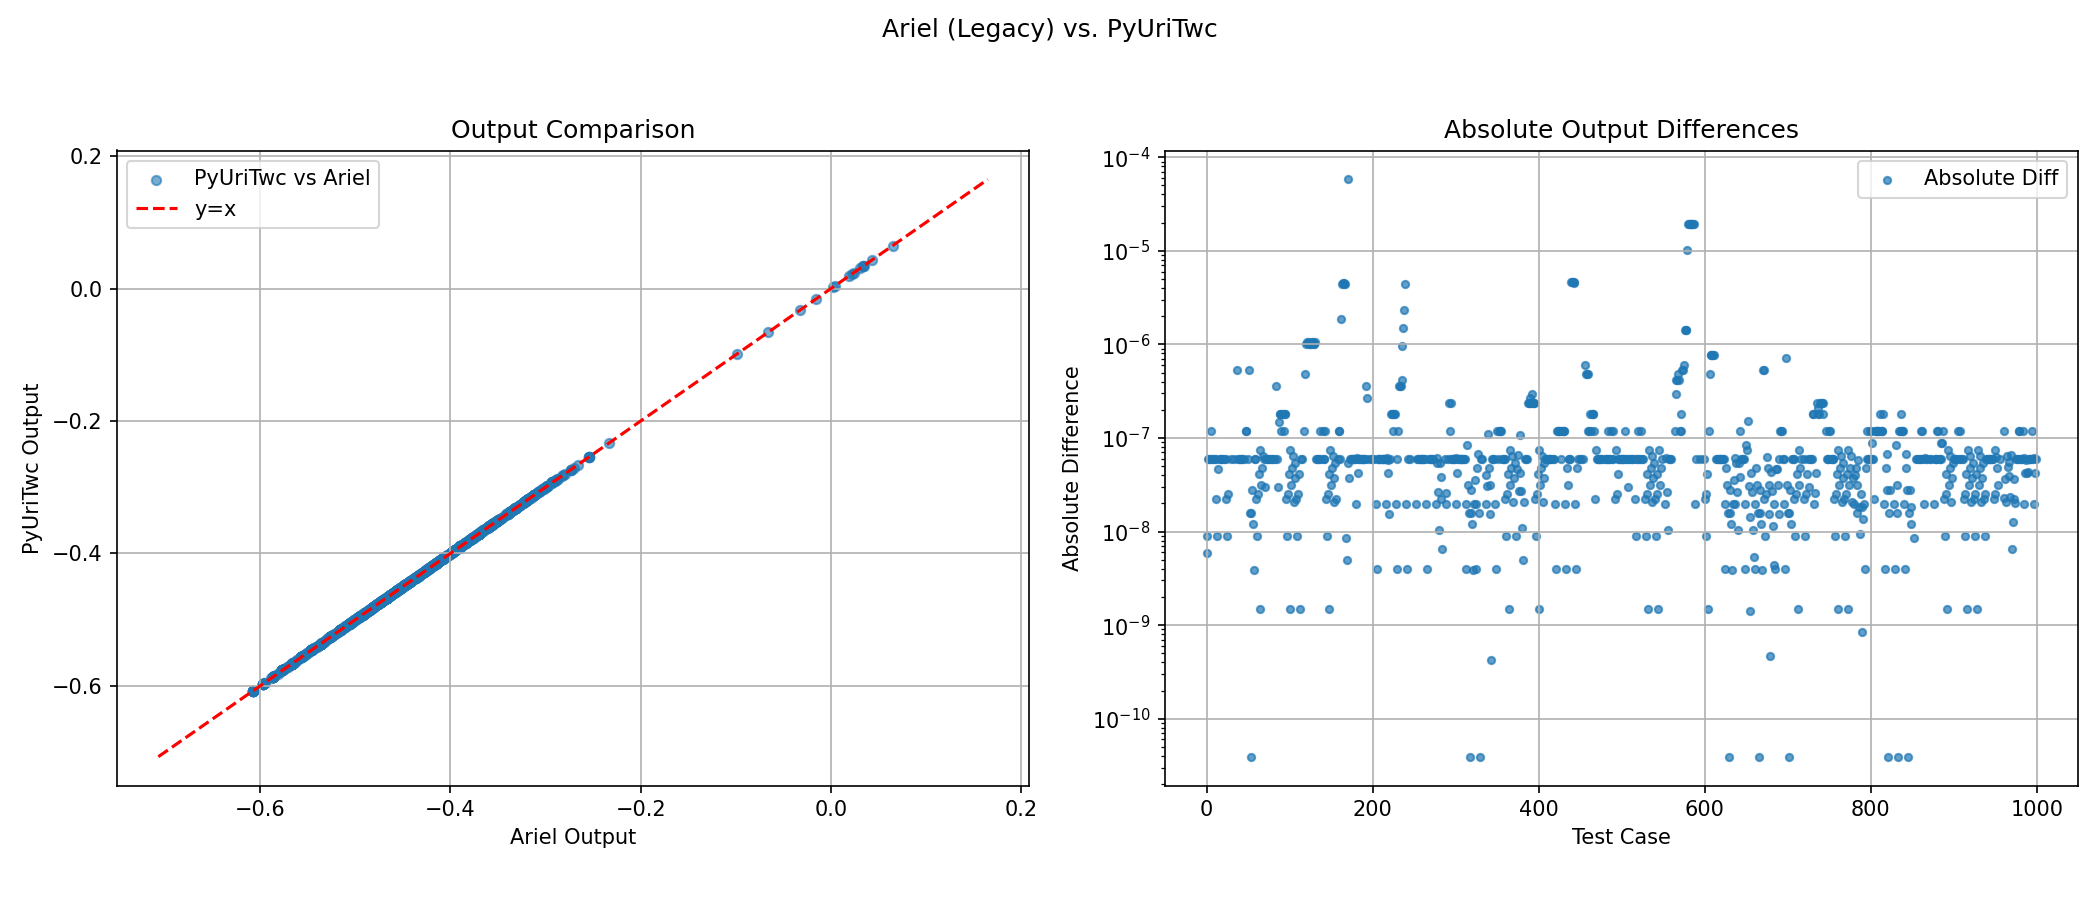
\includegraphics[
      width=\linewidth,
      height=0.82\textheight,
      keepaspectratio
    ]{./attatchments/pyuri_vs_ariel.png}
\end{frame}

\begin{frame}{Resultados de Referencia Publicados}
    \centering
    \small
    \setlength{\tabcolsep}{6pt}
    \renewcommand{\arraystretch}{1.15}
    \begin{table}
        \caption{Resultados reportados en la literatura}
        \begin{tabular}{l c c c c}
            \toprule
            \textbf{Modelo} &
            \textbf{Avg Recomp.} &
            \textbf{Std Recomp.} &
            \textbf{Avg Pasos} &
            \textbf{Std Pasos} \\
            \midrule
            FIU+RS & 98.43 & 0.15 & -- & -- \\
            \bottomrule
        \end{tabular}
    \end{table}
\end{frame}

\begin{frame}{Resultados Obtenidos}
    \centering
    \small % o \scriptsize si aún no entra
    \setlength{\tabcolsep}{3.5pt} % compacta columnas
    \renewcommand{\arraystretch}{1.15}

    \begin{table}
        \caption{Promedio sobre 100 episodios}
        \begin{tabularx}{\textwidth}{@{}l *{6}{>{\centering\arraybackslash}X}@{}}
            \toprule
            \textbf{Modelo} &
            \textbf{Avg Recomp.} &
            \textbf{Std Recomp.} &
            \textbf{Avg Pasos} &
            \textbf{Std Pasos} &
            \textbf{Avg Acción} &
            \textbf{Std Acción} \\
            \midrule

            \multicolumn{7}{@{}l}{\textit{Configuración 1}} \\
            \quad Mejor & \textbf{94.13} & 0.70 & 164.5 & 29.1 & 0.44 & 0.40 \\
            \quad Final & 94.04 & 0.64 & 158.6 & 30.9 & 0.45 & 0.42 \\
            \addlinespace[2pt]

            \multicolumn{7}{@{}l}{\textit{Configuración 2}} \\
            \quad Mejor & 93.14 & 0.36 & 156.8 & 25.8 & 0.51 & 0.42 \\
            \quad Final & 92.21 & 2.20 & 162.4 & 44.0 & 0.55 & 0.43 \\
            \addlinespace[2pt]

            \multicolumn{7}{@{}l}{\textit{Configuración 3}} \\
            \quad Mejor & 93.82 & 0.83 & 189.8 & 48.1 & 0.41 & 0.40 \\
            \quad Final & 92.84 & 1.24 & 175.3 & 38.2 & 0.48 & 0.42 \\
            \addlinespace[2pt]

            \textit{Referencia} & 93.64 & 0.74 & \textbf{124.5} & 6.1 & 0.61 & 0.36 \\
            \bottomrule
        \end{tabularx}
    \end{table}

\end{frame}

\begin{frame}{Demo}
    \centering
    \vspace{-0.15cm} % recupera un poco de espacio vertical
    \movie[
        width=0.85\textwidth,
        height=0.55\textheight,
        poster,
        loop
    ]{%
    \fbox{\parbox[c][0.55\textheight][c]{0.85\textwidth}{%
        \centering
        \Large ▶ Ver Demo
    }}
    }{attatchments/demo.mp4}
\end{frame}